\startchapter{Systematic Uncertainties}
\label{chapter:systematics}

In order to properly assess the significance of any discrepancies that may be seen between predicted yields and distributions of signal and SM background and the observed collision data, it is important to assign an uncertainties to all sources which may limit the precision and accuracy of the yield predictions. In addition to the limited precision of the estimates due to statistical uncertainty\footnote{See Chapter \ref{sec:mc_intro} for a discussion of the origin of statistical uncertainty in MC simulations.}, there may be inaccuracies in the values of various parameters involved in the simulation due to a limited precision with which their values are known. These inaccuracies can systematically shift predicted production rates and kinematic properties of the simulated processes, or the objects they produce in the ATLAS detector, and ultimately predicted yields and shapes of the processes in the analysis regions. Systematic uncertainties aim to quantify the maximal range of yield shifts, in each region and bin\footnote{See Section zzz \textcolor{red}{(Note to Bob: will update when section on binning is written)} for details of the binning in \minms performed in the SR} used in the search, that could result from a potential source of systematic inaccuracy. 

Systematic uncertainties (or simply ``systematics") are classified into two main categories: theoretical and experimental. Theoretical systematics account for inaccuracies that could result from a limited knowledge of parameters involved in modelling the production and decay mechanisms resulting from \(pp\) collision events at the LHC. Experimental systematics account for inaccuracies involved in the physics objects\footnote{See Section \ref{sec:object_defs} for a presentation of the reconstructed physics objects used in this search.} used to reconstruct the decay products of collision events in the ATLAS detector, and in the LHC machine itself. 

Experimental systematics are generally constrained in the process of calibrating particular physics objects reconstructed in the ATLAS detector using the ATLAS collision data, and as a result are generally considered quite robust. In contrast, the choice of an uncertainty to assign to theoretical parameters can be much less clear, as constraints from experimental results may be sparse, or in some cases such as appropriate choice of renormalization scale in perturbative QCD calculations \cite{PDG_2018}, essentially non-existent. 

\section{Experimental Systematics}

Experimental systematics are evaluated for all physics objects considered in the analysis, and for the LHC beam luminosity. 

The integrated luminosity \(\mathcal{L}_\text{int}\) recorded by the ATLAS detector for the full data set considered in this search is known with a precision of \(1.7\%\) \cite{ATLAS-CONF-2019-021}. Since, from Eq. \ref{eq:integrated_lumi}, the total number of recorded collision events scales linearly with the integrated beam luminosity, propagating this \(\pm1.7\%\) systematic to the yields results in coherent \(1.7\%\) up and down shifts in all bins of the predicted yields for all processes.

For a given systematic uncertainty on a parameter \(k\) in physics object, the general procedure for propagating the systematic uncertainty to the predicted yield \(N\) in a bin \(j\) is as follows:

\begin{itemize}
\item Repeat the reconstruction with \(p\) shifted up by one standard deviation: \(k\rightarrow k+\sigma_k\).
\item Evaluate the predicted yield in the bin \(N_\text{\(k\), up, bin \(j\)}\) with updated simulation. The ``up" systematic yield uncertainty is \(\text{syst}\text{( \(k\), up, bin \(j)\)} = N_\text{\(k\), up, bin \(j\)} - N_\text{nom, bin \(j\)}\), where \(N_\text{nom, bin \(j\)}\) is the nominal yield with the unshifted \(k\).
\item Repeat the above process with \(k\) shifted down by one standard deviation to evaluate the ``down" systematic uncertainty.
\end{itemize}

\noindent Due to the statistical uncertainties arising from the limited number of MC events available to propagate systematic shifts to associated yield shifts, asymmetries between the up and down yield shifts from the above procedure can occur simply due to statistical fluctuations in the number of events which fall into each bin, rather than from actual asymmetries in the underlying distribution of shifted yields. For this reason, the propagated yield systematics are symmetrized in each bin as follows:

\begin{equation}
\label{eq:exp_systs_symm}
\text{syst}\text{(exp \(k\), symm, bin \(j\))}= \pm\Bigg(\frac{N_\text{\(k\), up, bin \(j\)} - N_\text{\(k\), down, bin \(j\)}}{2}\Bigg)
\end{equation}

Table \ref{tab:exp_systs} summarizes the uncertainties considered for all physics objects in the search. 

\begin{table}
\centering
\caption{Sources of systematic uncertainty considered for all physics objects used in the search. }
\label{tab:exp_systs}
\footnotesize{
\begin{tabular}{l p{11cm}}
\toprule
\textbf{Physics Object} & \textbf{Systematic Uncertainties Considered} \\
\midrule
\midrule
Electrons & \(-\) Reconstruction, ID and isolation efficiency \newline \(-\) Energy scale and resolution \\
\midrule
Muons & \(-\) Reconstruction, ID and isolation efficiency \newline \(-\) Trigger efficiency \newline \(-\) Energy scale and resolution \newline \(-\) Track-to-vertex association \\
\midrule
\(R=0.4\) Jets & \(-\) Energy scale and resolution \newline \(-\) Quark flavour composition \newline \(-\) Jet-vertex association \newline \(-\) Pileup \newline \(-\) \btag efficiency \\
\midrule
TAR jets & \(-\) \(R=0.2\) subjets input to TAR algo \newline \phantom{xl} (consider same sources as for \(R=0.4\) jets) \newline \(-\) Uncertainties associated with tracks input to TAR algo \\
\midrule
\met & \(-\) Soft terms used in \met calculation \newline \(-\) Note that uncertainties associated with other objects used in \met \phantom{xxl}calculation are propagated to \met, so are not classified as \met \phantom{xxl}systematics. \\
\bottomrule
\end{tabular}}
\end{table}

Figure \ref{fig:exp_syst_shifts_bkg} shows the envelope of all symmetrized shifts in the total predicted yield from all SM backgrounds due to sources of systematics considered for each type of physics object in the merged and resolved SRs. Figure \ref{fig:exp_syst_shifts_sig} shows the same set of envelopes for a sample signal point at \((\ms, \mZp)=(210, 2100)~\GeV\). Comparing the yield shifts associated with the reconstruction of the various physics objects, the experimental systematics are dominated by sources of uncertainty associated with the reconstruction of \(R=0.4\) jets and \(R=0.2\) TAR subjets in the merged SR. The \(R=0.2\) TAR subjets uncertainties produce relatively small yield shifts in the resolved SR because TAR jets are not used in this region. Shifts in predicted yield are also noticeably smaller for the signal model compared with the SM background processes. This is likely due to the larger number of MC simulated events which are admitted into the SRs for the signal process, and the consequently smaller relative statistical fluctuations in yield shifts due to varying sources of uncertainty in the object reconstruction.

\begin{figure}[htbp]
  \centering
    \begin{subfigure}[t]{0.48\textwidth}
    \centering
     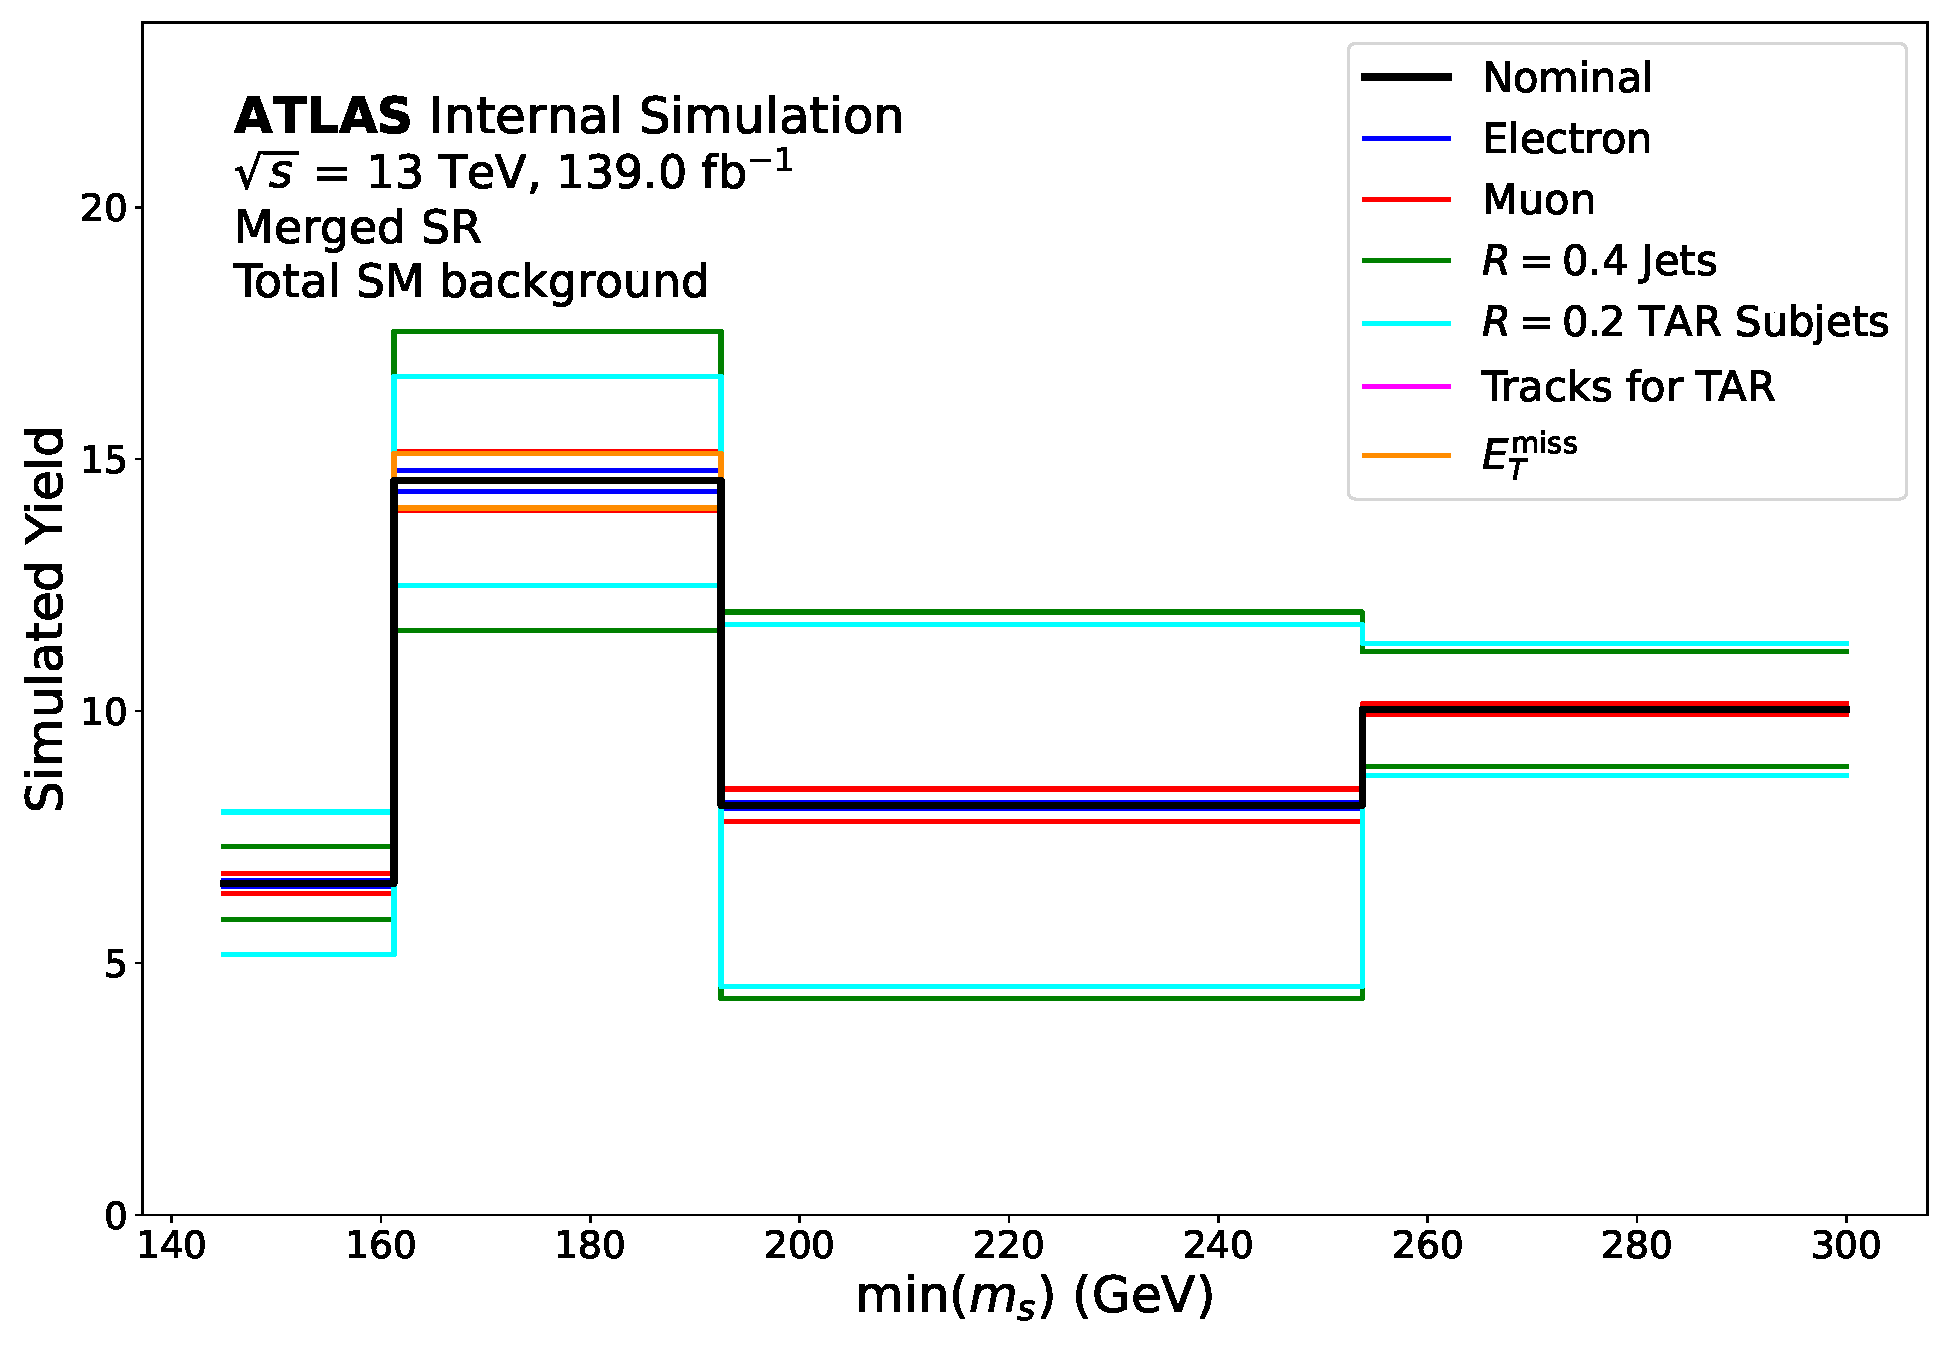
\includegraphics[width = 0.99\textwidth]{Figures/6/exp_systs_total_bkg_SR_mgd_TARJets10_minmS_mgd.pdf}
    \caption{Merged SR}
    \end{subfigure}
    \begin{subfigure}[t]{0.48\textwidth}
    \centering
     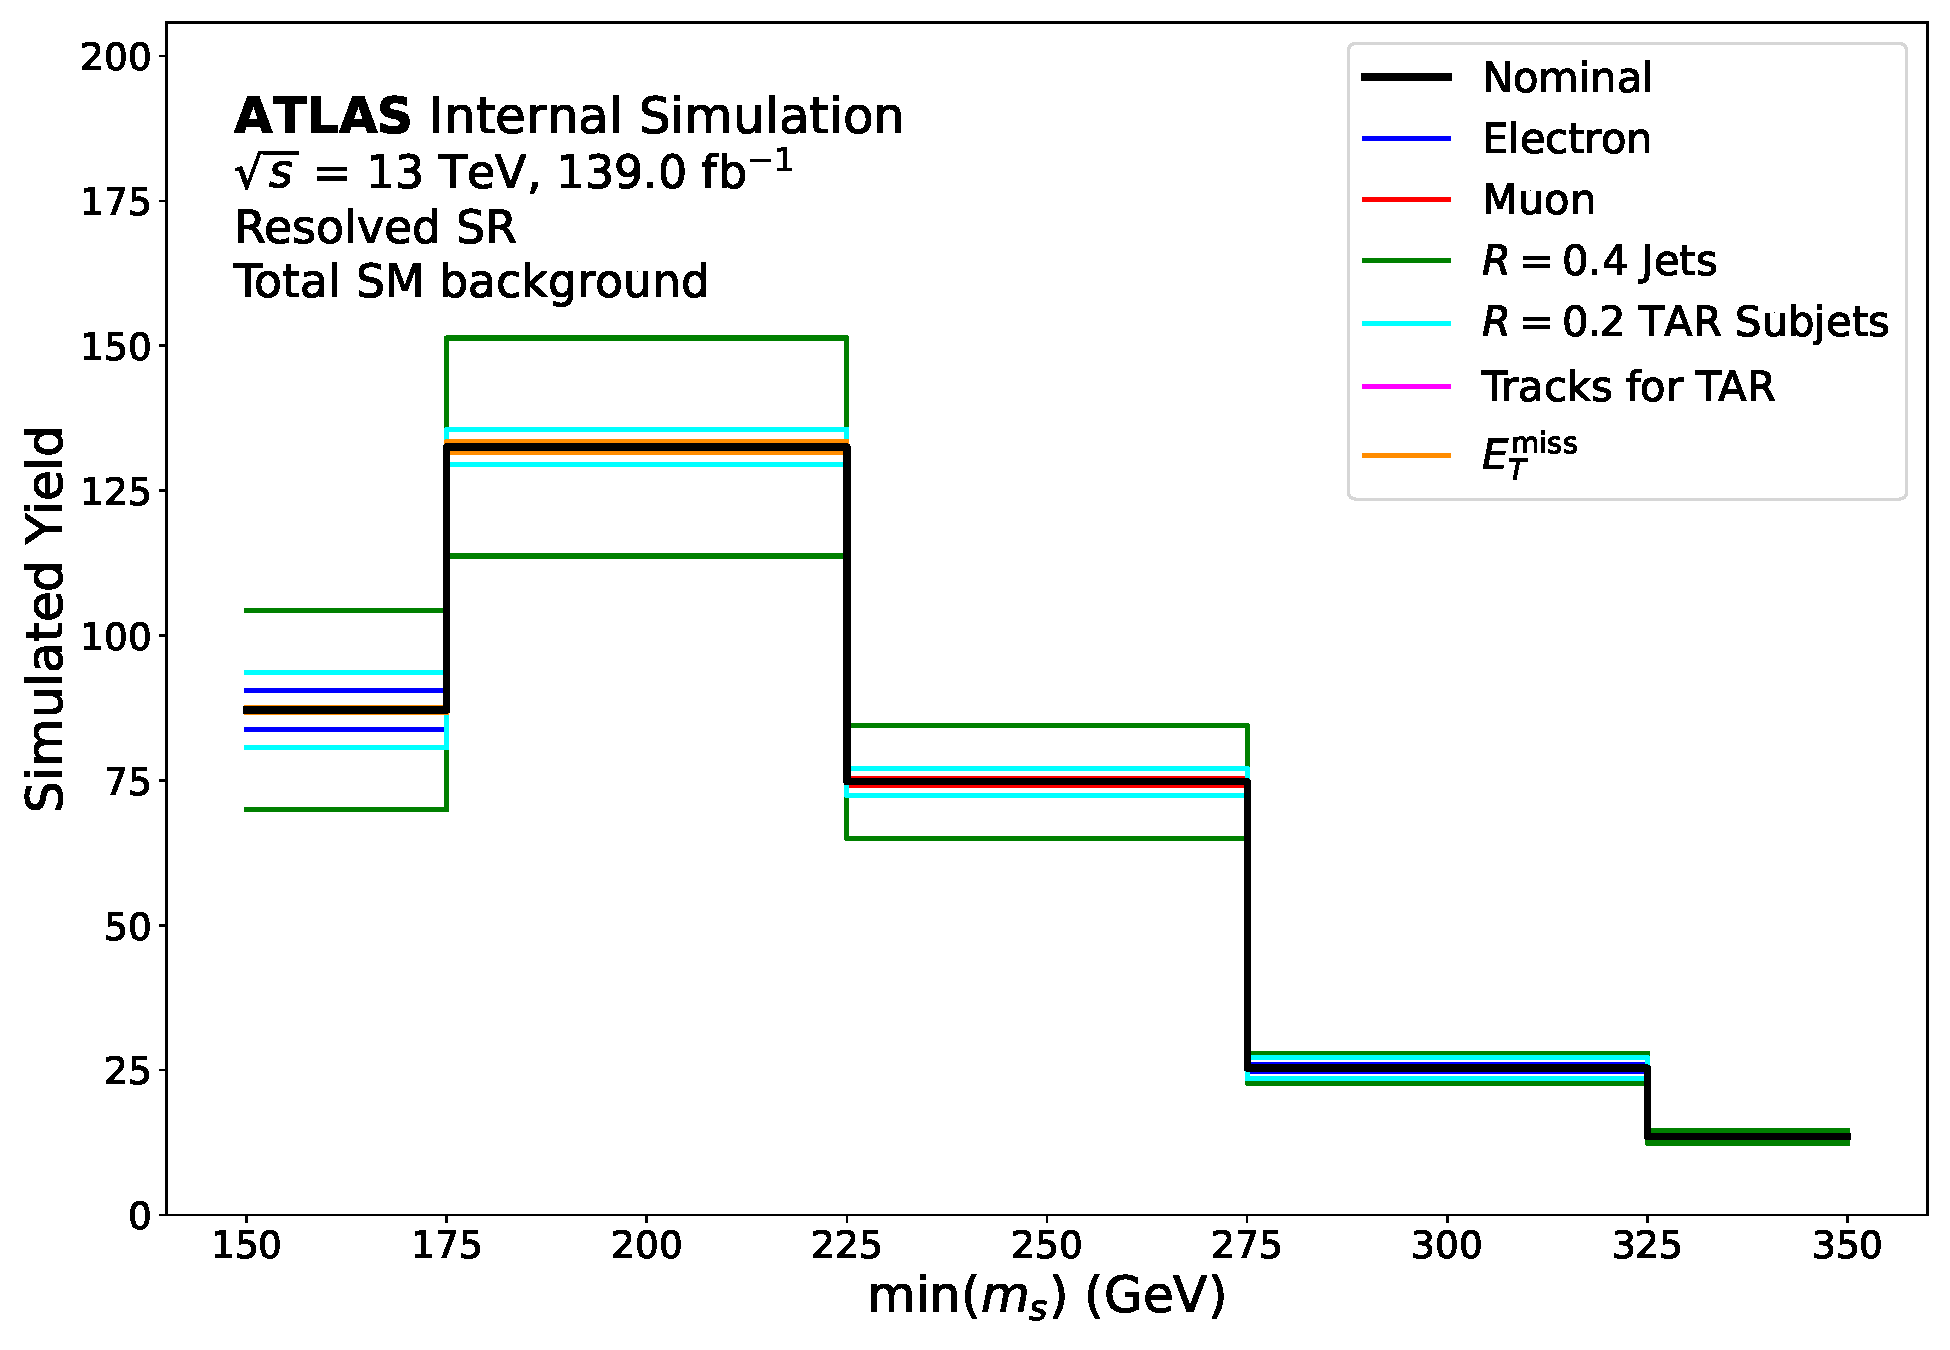
\includegraphics[width = 0.99\textwidth]{Figures/6/exp_systs_total_bkg_SR_res_TARJets10_minmS_res.pdf}
     \caption{Resolved SR}
    \end{subfigure}
    \caption{Envelope of shifts in the total predicted yield of SM background processes in the merged (left) and resolved (right) SRs due to experimental systematics associated with each physics object considered in the search. The predicted yield is binned in \minms using the binning strategy employed in the fitting strategy to search for evidence of the DH signal model in the data (see Chapter \ref{chapter:stat} for details). }
   \label{fig:exp_syst_shifts_bkg}
\end{figure}

\begin{figure}[htbp]
  \centering
    \begin{subfigure}[t]{0.48\textwidth}
    \centering
     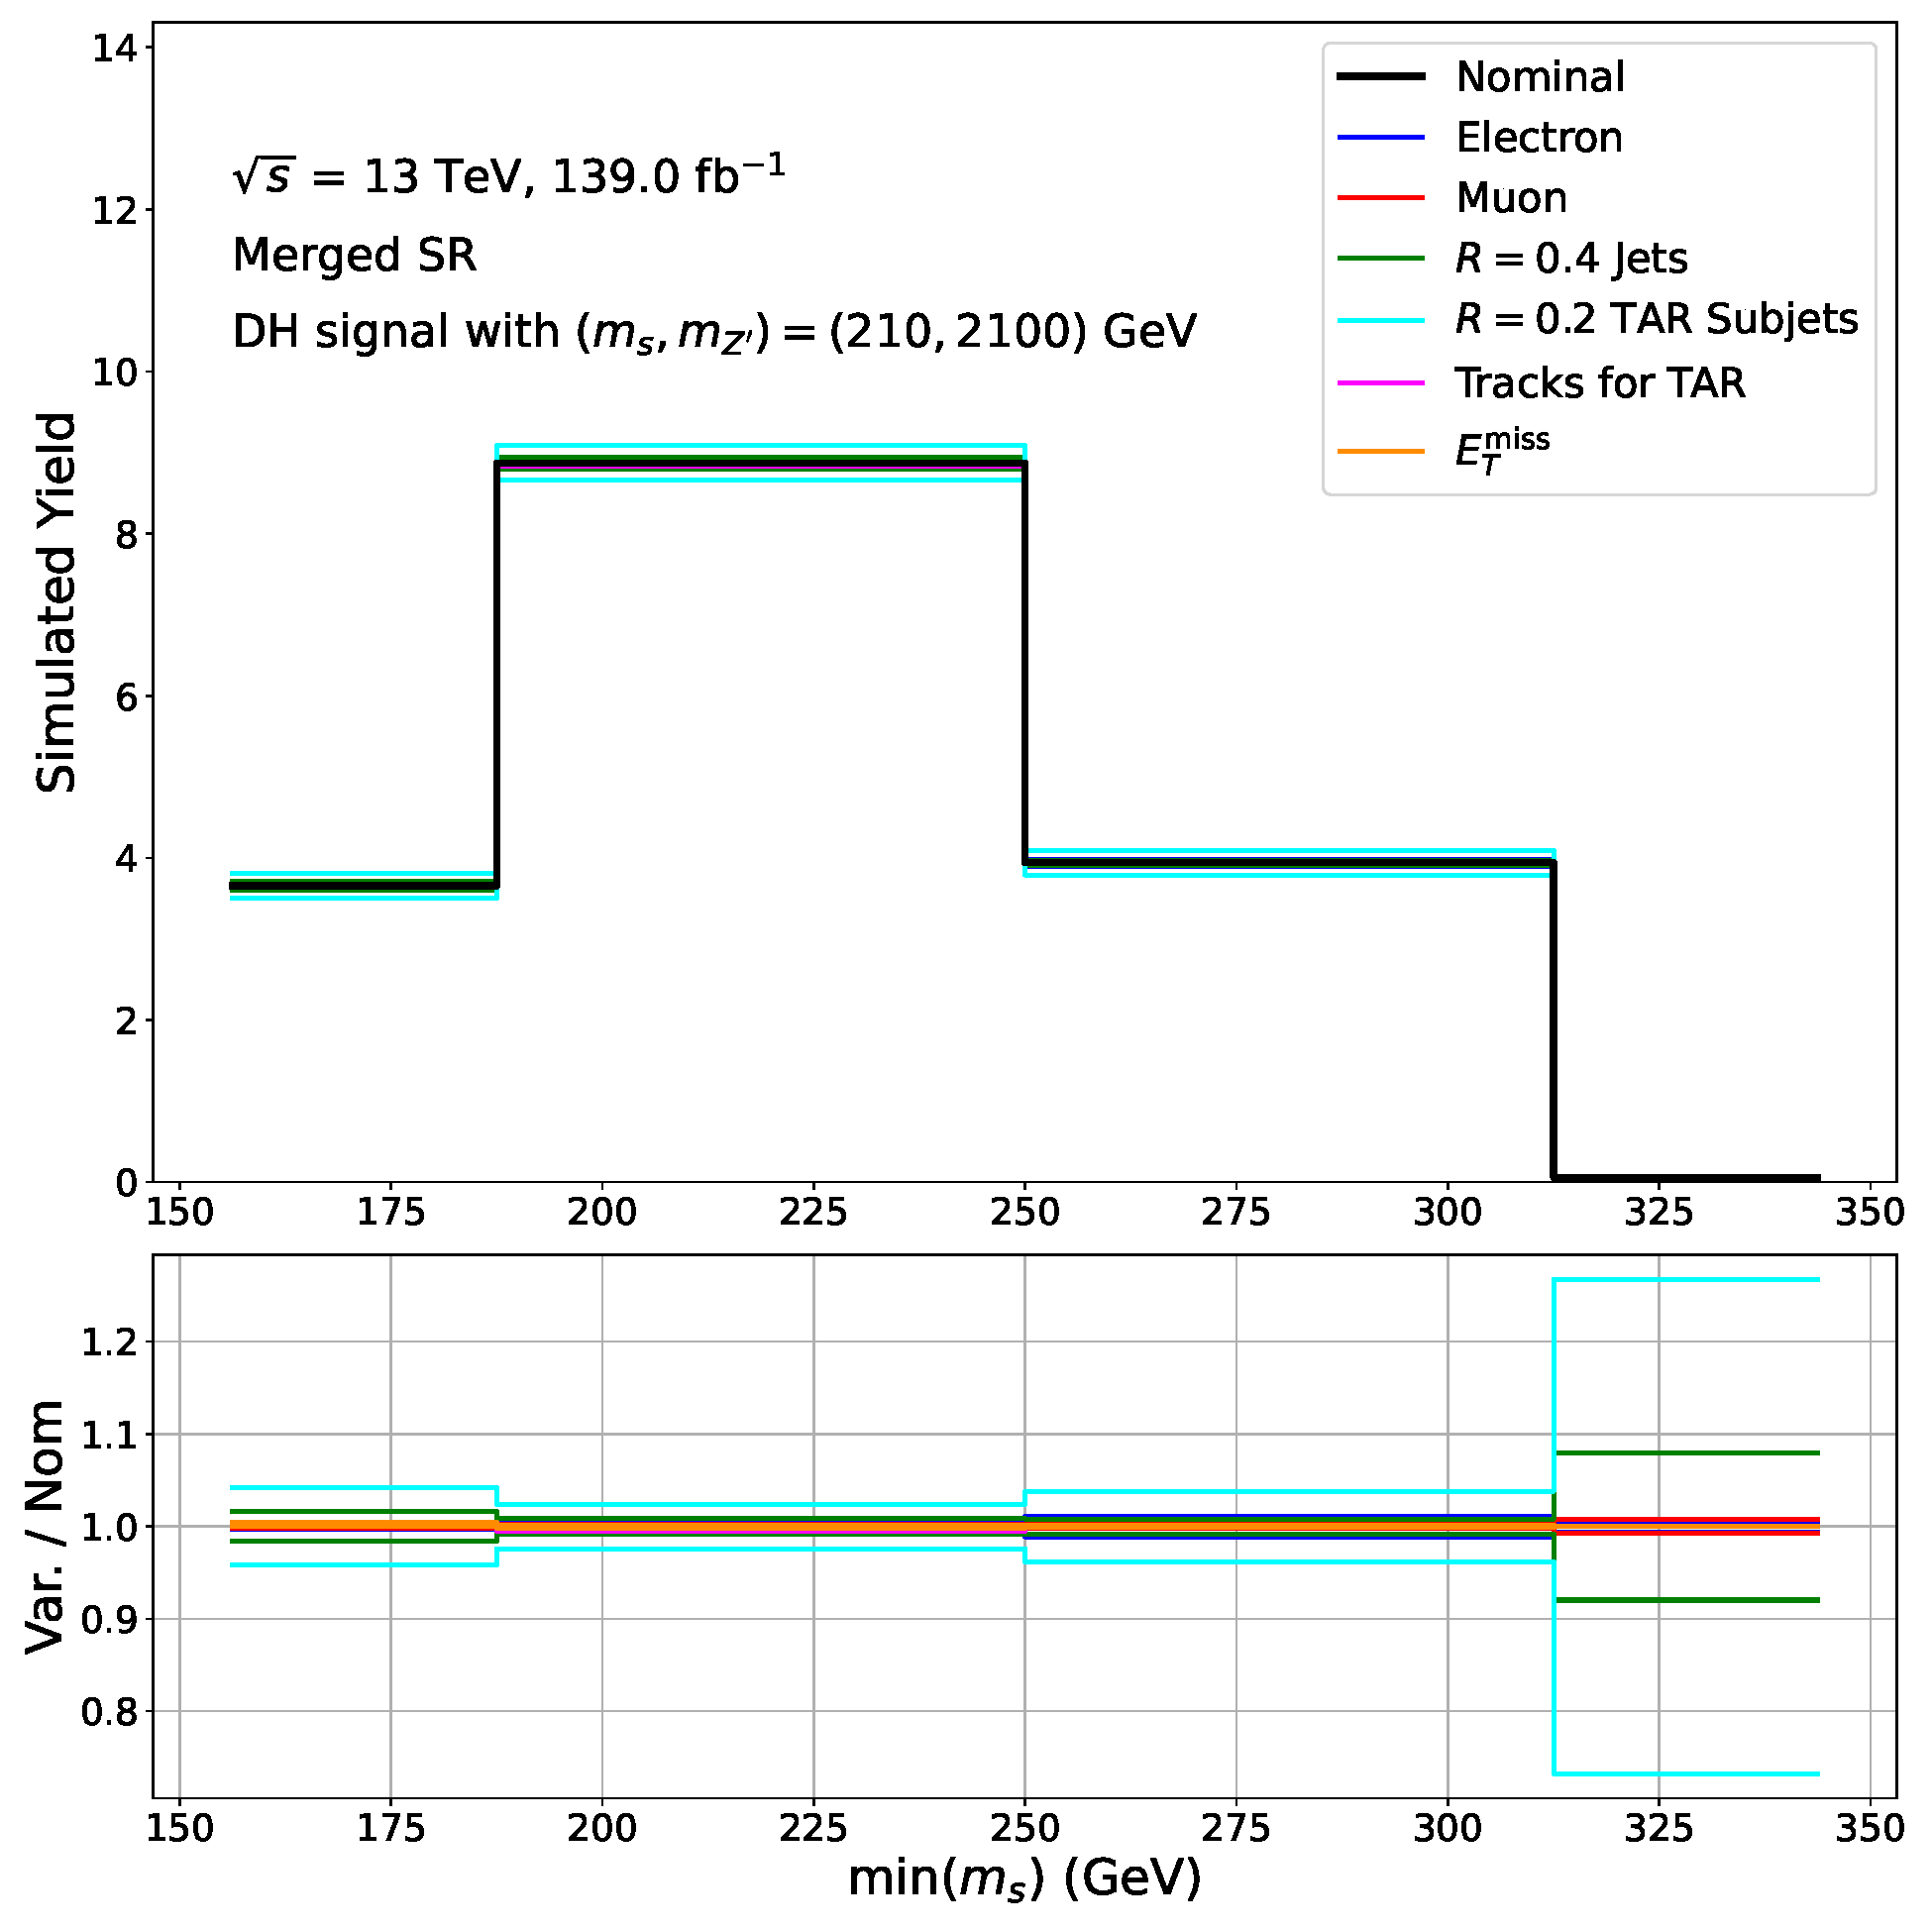
\includegraphics[width = 0.99\textwidth]{Figures/6/exp_systs_monoSWWsemilep_zp2100_dm200_dh210_SR_mgd_TARJets10_minmS_mgd.pdf}
    \caption{Merged SR}
    \end{subfigure}
    \begin{subfigure}[t]{0.48\textwidth}
    \centering
     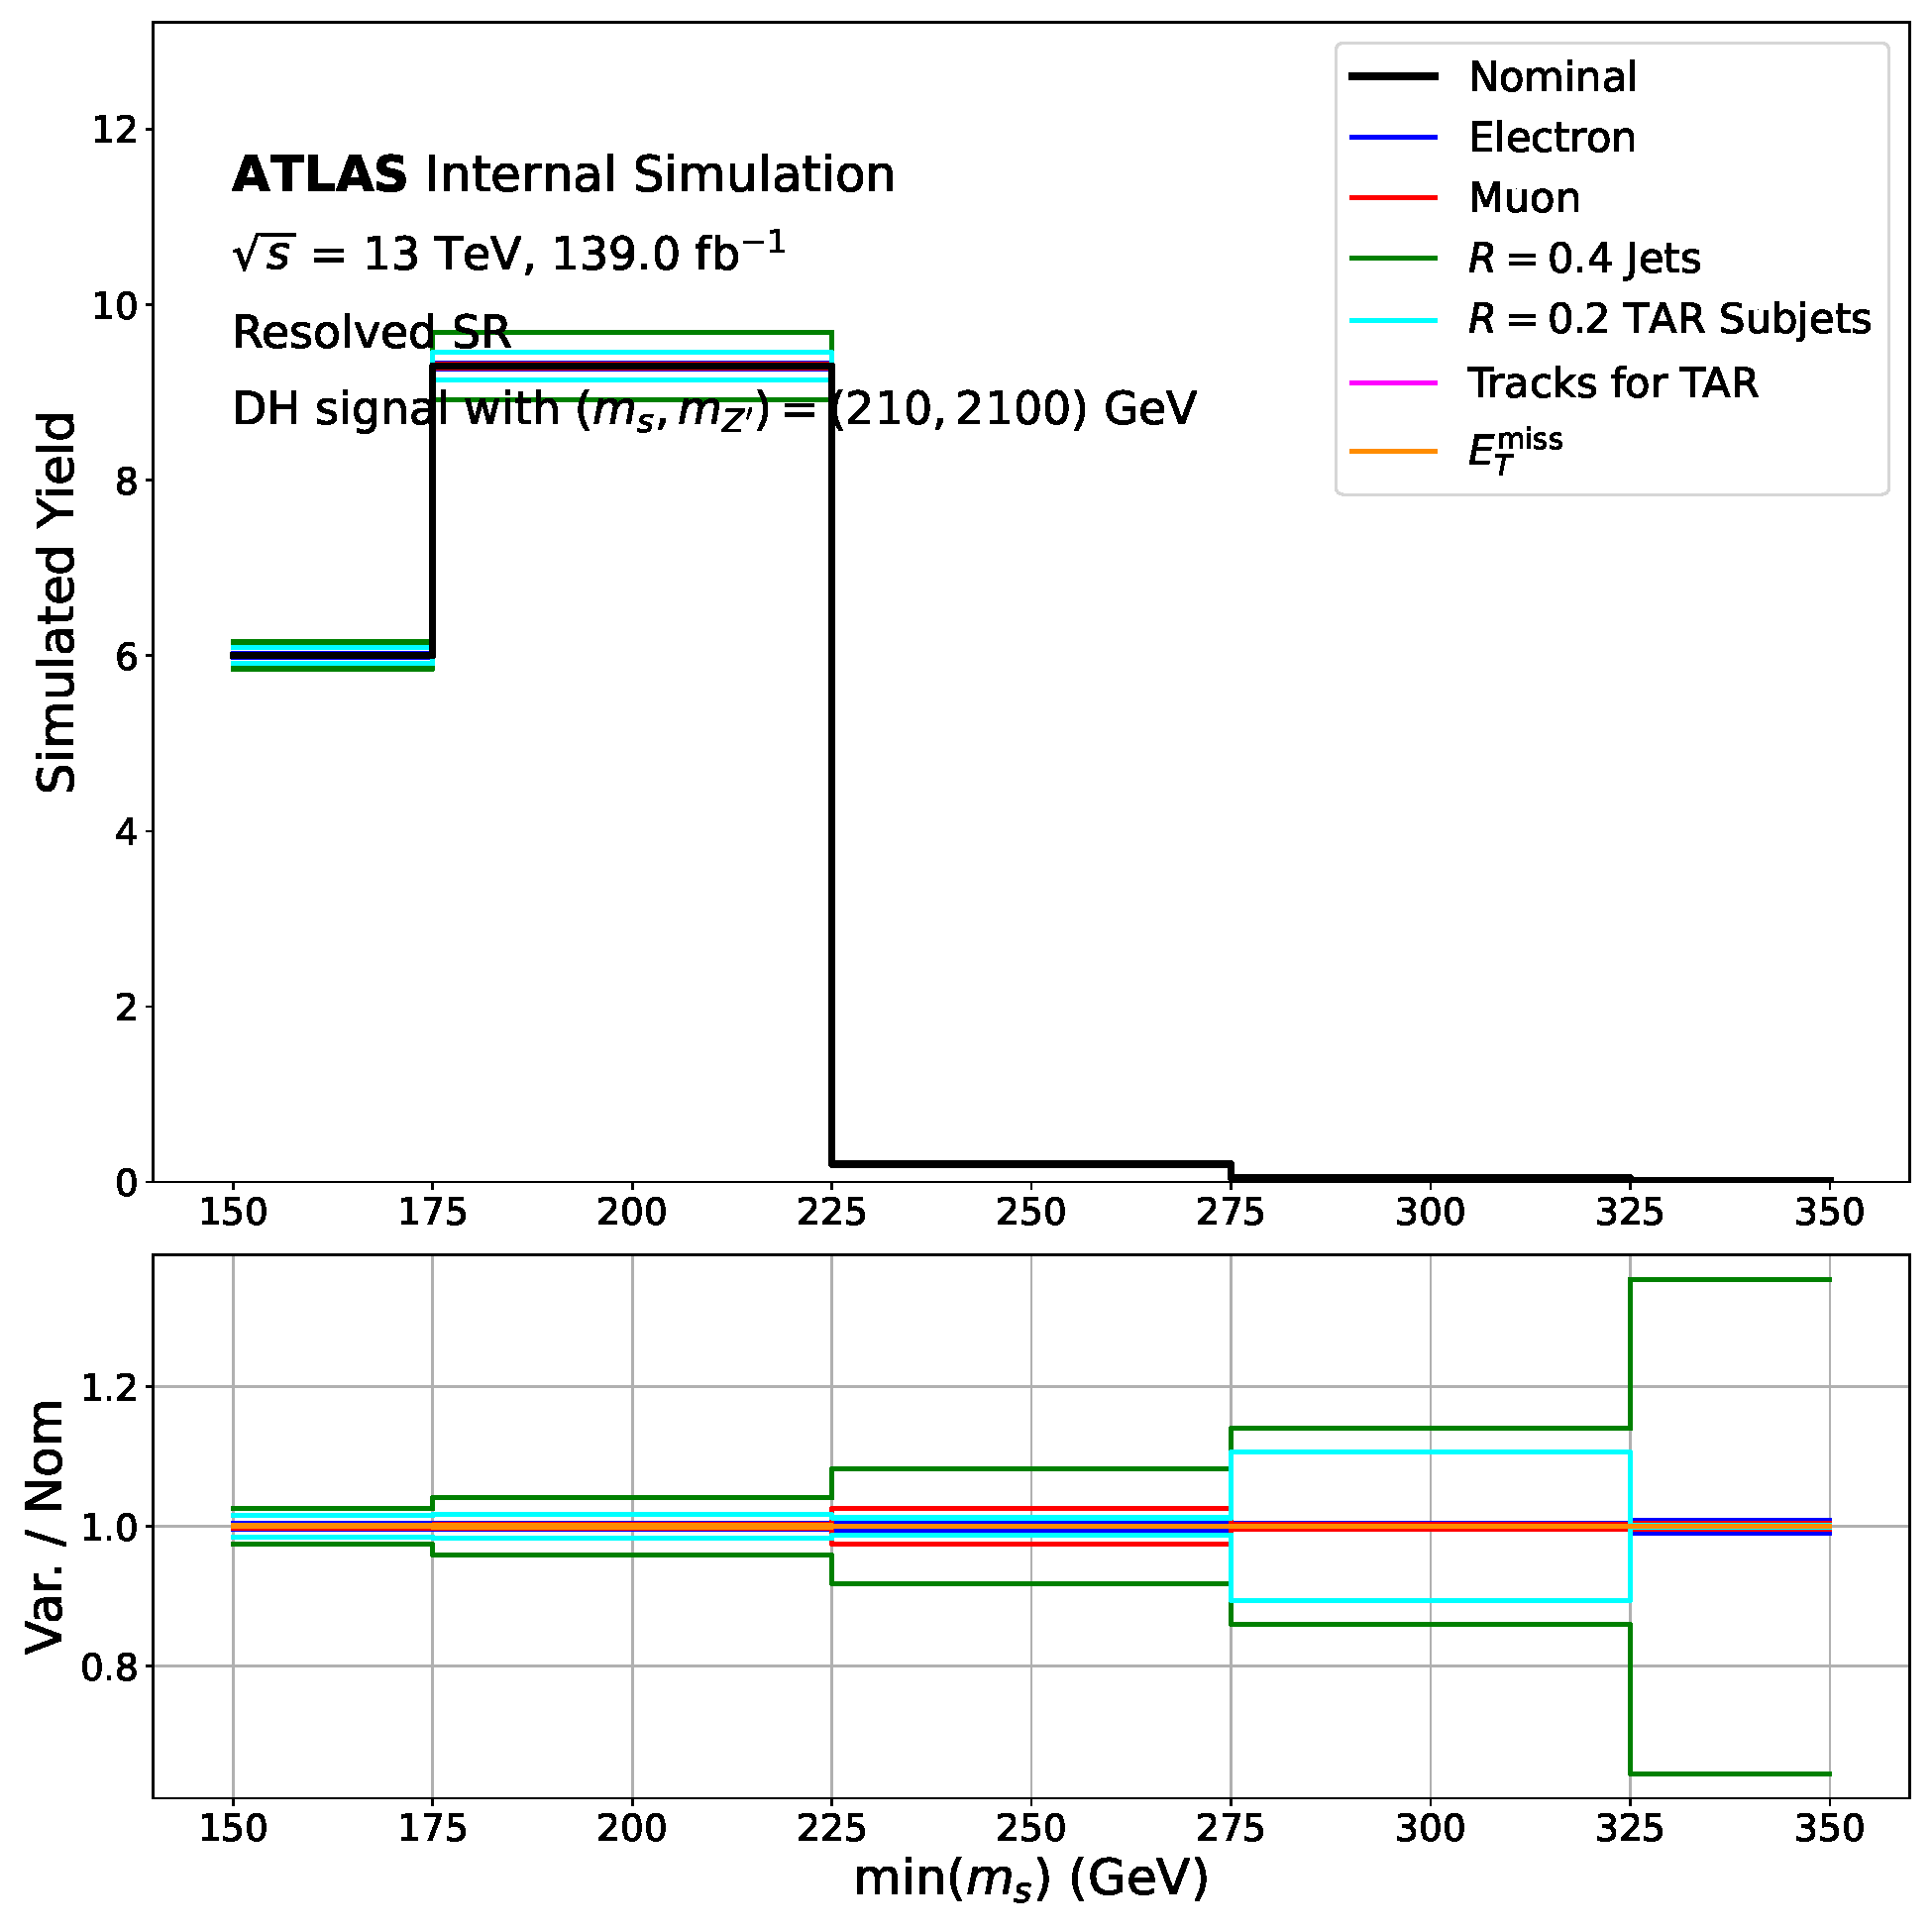
\includegraphics[width = 0.99\textwidth]{Figures/6/exp_systs_monoSWWsemilep_zp2100_dm200_dh210_SR_res_TARJets10_minmS_res.pdf}
     \caption{Resolved SR}
    \end{subfigure}
    \caption{Envelope of shifts in the predicted yield of the DH signal process at \((\ms, \mZp)=(210, 2100)\) in the merged (left) and resolved (right) SRs due to experimental systematics associated with each physics object considered in the search. The predicted yield is binned in \minms using the binning strategy employed in the fitting strategy to search for evidence of the DH signal model in the data (see Chapter \ref{chapter:stat} for details). }
   \label{fig:exp_syst_shifts_sig}
\end{figure}

Tables \ref{tab:systs_total_bkg_JET_JER_SR} and \ref{tab:systs_total_bkg_JET_JER_CR} show a sample breakdown of the up/down systematic shifts in the total predicted yield of SM background processes in the SRs and CRs, respectively, which arise from shifting parameters associated with the jet energy resolution of \(R=0.4\) jets by \(\pm\sigma\). 

\begin{table}[ht]
\caption{\label{tab:systs_total_bkg_JET_JER_SR} Symmetrized up and down uncertainties in total predicted yield of all SM background processes in the merged and resolved SRs due to varying parameters associated with jet energy resolution (JER) by \(\pm1\sigma\). Uncertainties are reported as percent shift relative to nominal yield.}
\footnotesize{
\begin{tabular}{l l l l l }
\toprule
\textbf{Name of JER parameter} & \textbf{Mgd SR} & \textbf{Res SR}\tabularnewline
\midrule
\midrule
JET\_JER\_DataVsMC\_MC16 & \(\pm\)6.09\% &\(\pm\)1.17\% \tabularnewline
\midrule
JET\_JER\_EffectiveNP\_1 & \(\pm\)8.74\% &\(\pm\)0.07\% \tabularnewline
\midrule
JET\_JER\_EffectiveNP\_2 & \(\pm\)2.62\% &\(\pm\)2.73\% \tabularnewline
\midrule
JET\_JER\_EffectiveNP\_3 & \(\pm\)0.48\% &\(\pm\)0.87\% \tabularnewline
\midrule
JET\_JER\_EffectiveNP\_4 & \(\pm\)0.83\% &\(\pm\)1.66\% \tabularnewline
\midrule
JET\_JER\_EffectiveNP\_5 & \(\pm\)4.59\% &\(\pm\)3.70\% \tabularnewline
\midrule
JET\_JER\_EffectiveNP\_6 & \(\pm\)7.59\% &\(\pm\)2.44\% \tabularnewline
\midrule
JET\_JER\_EffectiveNP\_7restTerm & \(\pm\)2.96\% &\(\pm\)0.60\% \tabularnewline
\bottomrule
\end{tabular}}
\end{table}

\begin{table}[ht]
\caption{\label{tab:systs_total_bkg_JET_JER_CR} Symmetrized up and down uncertainties in total predicted yield of all SM background processes in the merged and resolved CRs due to varying parameters associated with jet energy resolution (JER) by \(\pm1\sigma\). Uncertainties are reported as percent shift relative to nominal yield.}
\footnotesize{
\begin{tabular}{l l l l l }
\toprule
\textbf{Name of JER parameter} & \textbf{Mgd CRW} & \textbf{Res CRW} & \textbf{Mgd CRTT} & \textbf{Res CRTT}\tabularnewline
\midrule
\midrule
JET\_JER\_DataVsMC\_MC16 & \(\pm\)0.42\% &\(\pm\)0.98\% &\(\pm\)1.25\% &\(\pm\)1.57\% \tabularnewline
\midrule
JET\_JER\_EffectiveNP\_1 & \(\pm\)0.75\% &\(\pm\)0.68\% &\(\pm\)1.07\% &\(\pm\)4.50\% \tabularnewline
\midrule
JET\_JER\_EffectiveNP\_2 & \(\pm\)0.77\% &\(\pm\)0.82\% &\(\pm\)0.73\% &\(\pm\)6.47\% \tabularnewline
\midrule
JET\_JER\_EffectiveNP\_3 & \(\pm\)0.56\% &\(\pm\)1.31\% &\(\pm\)1.05\% &\(\pm\)4.10\% \tabularnewline
\midrule
JET\_JER\_EffectiveNP\_4 & \(\pm\)0.89\% &\(\pm\)2.91\% &\(\pm\)0.13\% &\(\pm\)4.09\% \tabularnewline
\midrule
JET\_JER\_EffectiveNP\_5 & \(\pm\)0.55\% &\(\pm\)0.61\% &\(\pm\)0.24\% &\(\pm\)6.29\% \tabularnewline
\midrule
JET\_JER\_EffectiveNP\_6 & \(\pm\)0.03\% &\(\pm\)1.61\% &\(\pm\)0.32\% &\(\pm\)5.69\% \tabularnewline
\midrule
JET\_JER\_EffectiveNP\_7restTerm & \(\pm\)0.21\% &\(\pm\)1.72\% &\(\pm\)0.03\% &\(\pm\)4.29\% \tabularnewline
\bottomrule
\end{tabular}}
\end{table}

\section{Theoretical Systematics}

The sources of theoretical uncertainty considered in this search, as well as the methods used to evaluate the resulting uncertainties in predicted yields for the various processes relevant to the search, are discussed in the following sections.  Some sources are only considered for a subset of the processes. Table \ref{tab:theo_sys_summary} summarizes the theoretical uncertainties that are evaluated for each process.

\begin{table}
\centering
\caption{}
\label{tab:theo_sys_summary}
%\begin{tabular}{l p{6cm} l l }
\footnotesize{
\begin{tabular}{l l l l l l l l }
\toprule
\textbf{Uncertainty Source} & \textbf{W+jets} & \textbf{Diboson} & \textbf{Triboson} & \textbf{Z+jets} & \(\mathbf{\ttbar}\) & \textbf{Single Top} & \textbf{DH Signal} \\
\midrule
\midrule
PDF & \checkmark & \checkmark & \checkmark & \checkmark & \checkmark & \checkmark \\
\midrule
\(\alpha_s\) (PDF) & \checkmark & \checkmark & \checkmark & \checkmark & \(\times\) & \(\times\) & \(\times\) \\
\midrule
\(\alpha_s\) (ISR) & \(\times\) & \(\times\) & \(\times\) & \(\times\) & \checkmark & \checkmark & \(\times\) \\
\midrule
QCD \(\mu_R\) and \(\mu_F\) & \checkmark & \checkmark & \checkmark & \checkmark & \checkmark & \checkmark & \checkmark \\
\midrule
Matrix Element & \(\times\) & \(\times\) & \(\times\) & \(\times\) & \checkmark & \checkmark & \(\times\) \\
\midrule
Parton Showering & \checkmark & \checkmark & \checkmark & \checkmark & \checkmark & \checkmark & \checkmark \\
\midrule
\ttbar/\(Wt\) Interference & \(\times\) & \(\times\) & \(\times\) & \(\times\) & \(\times\) &  \(\times\) & \checkmark \\
\bottomrule
\end{tabular}}
\end{table}

\subsection{Modelling the Parton Distribution Function}
\label{sec:pdf_unc}

Uncertainties associated with the parton distribution functions\footnote{See Section \ref{sec:parton_model} for an introduction to the parton model and parton distribution functions.} (PDF) used to model the substructure of protons involved in LHC collisions can affect cross sections - and hence production rates - of production and decay processes at the LHC. Following ATLAS guidelines and recommendations from the \textit{PDF4LHC} \cite{PDF4LHC_recos_2016} working group, generator weights\footnote{See discussion of generator weights in Section \ref{sec:evt_wts}} for all simulated events are re-evaluated for 100 replicas of the nominal PDF. Each replica is obtained by randomly re-sampling all uncertain inputs to the model and re-evaluating the PDF with the new inputs \cite{BALL20091}. The yield in each region and bin is re-evaluated with each set of generator weights, and the uncertainty of the yield in each bin is estimated as the standard deviation over all yield variations.

\subsection{Strong Coupling Constant \(\alpha_s\)}

The nominal PDF is produced with the strong coupling constant \(\alpha_s\) set to its currently accepted value of \(alpha_s(m_Z^2)=0.1180\pm0.0015\) \cite{PDF4LHC_recos_2016} at a momentum scale \(m_Z\). 

\subsubsection{\(\alpha_s\) in PDF Modelling}

For the \wjets, \zjets, diboson and triboson processes generated using \SHERPA, alternative generator weights are produced using PDFs re-evaluated with \(\alpha_s\) varied up or down by its \(\pm0.0015\) uncertainty. Following the \textit{PDF4LHC} prescription, yield \(N_p\) for a given process \(p\) is re-evaluated in each bin \(j\) with the alternative generator weights, and the uncertainty is evaluated as:

\begin{equation}
\label{eq:alphas_syst}
\text{syst}\text{(\(\alpha_s\), bin \(j\))}= \pm\Bigg(\frac{N_\text{\(p\), \(\alpha_s\)+1\(\sigma\), bin \(j\)} - N_\text{\(p\), \(\alpha_s\)-1\(\sigma\), bin \(j\)} }{2}\Bigg)
\end{equation}

\noindent and added in quadrature with the PDF uncertainties described in Section \ref{sec:pdf_unc}.

\subsubsection{Strong Coupling Constant in the Modelling of ISR}

For the single-top and \ttbar processes generated using the \POWHEGBOX matrix element generator interfaced with the \PYTHIA8 parton shower generator, the effect of varying the strong \(\alpha_s\) used to model initial state radiation from 0.1-0.15 is evaluated using the up and down Var3c A14 tune variation \cite{ATL-PHYS-PUB-2014-021}, and the associated yield uncertainty in each bin is evaluated as half the resulting difference of yields, as in Eq. \ref{eq:alphas_syst}. 

\subsection{Renormalization and Factorization Scales (\(\mu_R\) and \(\mu_F\)) in QCD}

In the framework of perturbative QCD, the strong coupling constant is expressed as a function of the ``renormalization scale" \(\mu_R\) \cite{PDG_2018}, which is unphysical in the sense that the values of physical observables should be independent of \(\mu_R\). However, the choice of \(\mu_R\) can impact the calculated values of observables in perturbative QCD calculations due to missing higher-order terms in truncated expansions. A similar effect is seen with the ``factorization scale" \(\mu_F\) used in PDF calculations \cite{maltoni2007choosing}, which effectively quantifies the resolution with which the proton is probed in a collision. As with \(\mu_R\), the choice of \(\mu_F\) is physically meaningless, but affects the calculated values of observables due to missing higher-order terms in truncated QCD expansions.

To account for the unphysical impact of the choice of \(\mu_R\) and \(\mu_F\), generator weights are re-evaluated for each process with \(\mu_R\) and \(\mu_F\) varied by factors of either \(\frac{1}{2}\) or 2 in pairwise combinations (i.e. \((\mu_R, \mu_F)\rightarrow \{(\frac{1}{2}\mu_R, \mu_F), (\mu_R, 2\mu_F)\}\), etc.) from their values used for the nominal event generation. Following ATLAS guidelines, the systematic uncertainty in the yield in each bin is evaluated as the envelope of yield variations over all pairwise combinations of \(\mu_R\) and \(\mu_F\) variations, excluding the extreme off-diagonals \(\{(\frac{1}{2}\mu_R, 2\mu_F), (2\mu_R, \frac{1}{2}\mu_F)\}\).

\subsection{Matrix Element Generator Comparison}

\subsection{Parton Showering}



\subsection{Interference Between single-top and \ttbar Processes at NLO}

\begin{itemize}
\item Discussion of the sources of theory systematics considered (QCD scale, PDF, $\alpha_s$, PS) and how each is evaluated for signal and background.
\item Plots and tables showing the yield shifts and relative sizes of each source of theory uncertainty for signal and major backgrounds.
\item Comparison of the relative impact of statistical vs. systematic uncertainties in each analysis region, to identify where we're stats- vs. systematics-dominated.
\end{itemize}